\subsection{Results}
\label{sec:results}

\newcommand{\takeaway}[1]{
\vspace{6pt}
\noindent\fbox{\parbox{0.98\columnwidth}{#1}}
\vspace{6pt}
}

\begin{figure}
  \centering
  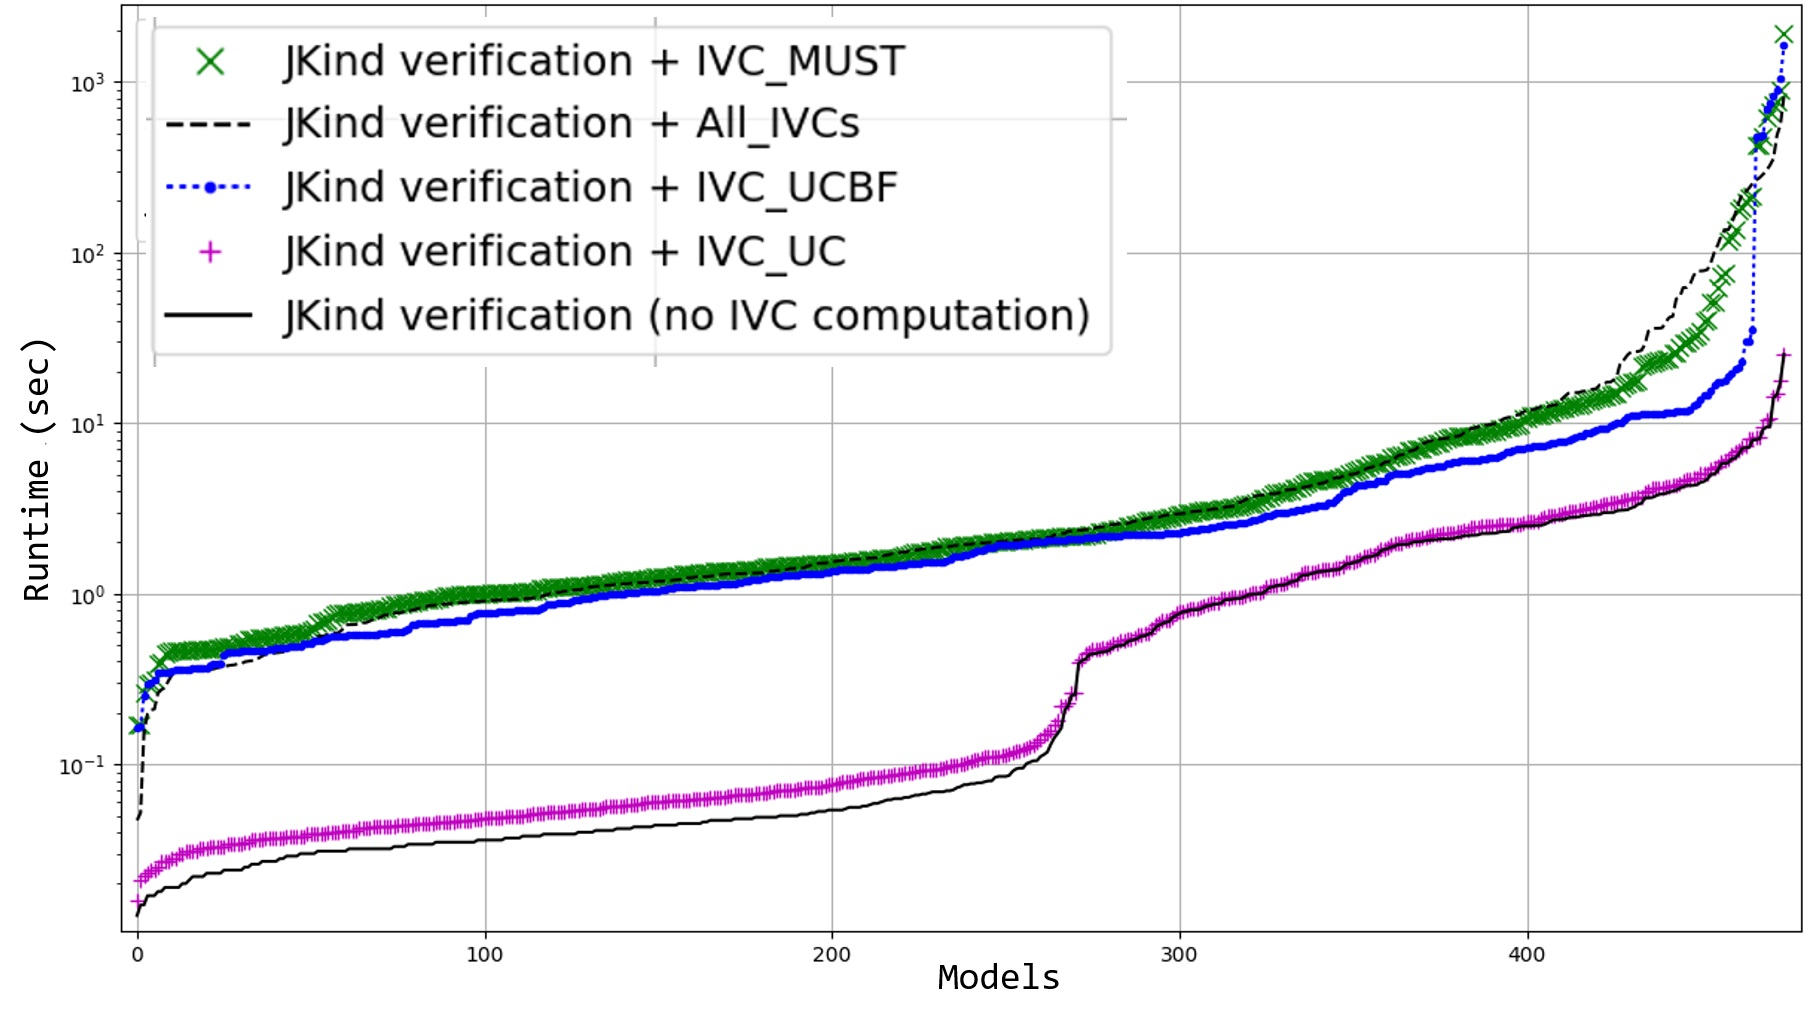
\includegraphics[width=\columnwidth]{figs/timing_analyses_all_sorted.jpg}
  \vspace{-0.1in}
  \caption{Runtime of different analyses}\label{fig:runtimeall}
\end{figure}

\begin{figure}
  \centering
  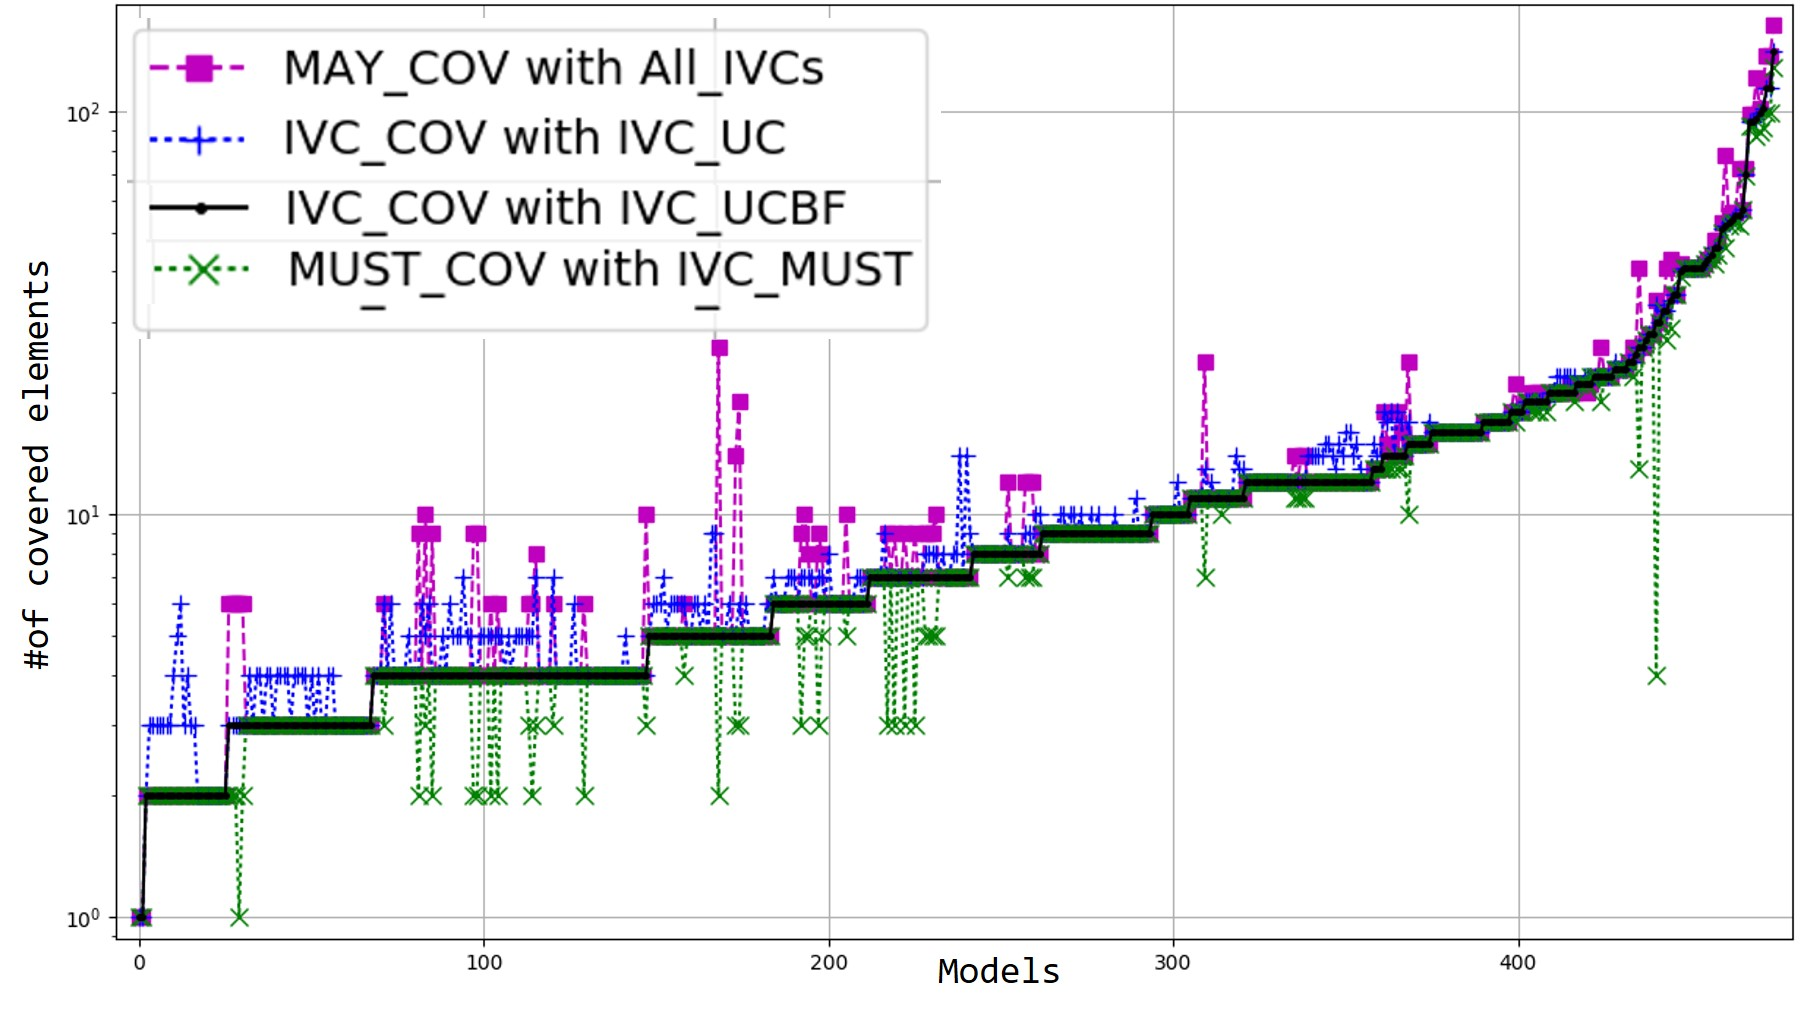
\includegraphics[width=\columnwidth]{figs/size.jpg}
  \vspace{-0.1in}
  \caption{Size of the set of covered elements by different algorithms}\label{fig:size}
\end{figure}

In this section, we examine our experimental results to address the research questions stated in \ref{sec:experiments}.

\textbf{RQ1:} First we examine the performance overhead of the \ucalg algorithm over the time necessary to find a proof using inductive model checking. To measure the performance overhead of an algorithm, we executed it over the proof generated by the {\em fastest} of the parallel \texttt{JKind} proof engines (k-induction, PDR, or invariant-generation). Tables~\ref{tab:runtime-ucalg}
and~\ref{tab:overhead-ucalg} represent both the
computation time for coverage analysis
and the overhead imposed by the algorithms.

\begin{table}
  \caption{runtime of different coverage analyses}
  \centering
  \begin{tabular}{ |c||c|c|c|c| }
    \hline
     runtime (sec) & min & max & mean & stdev \\[0.5ex]
    \hline\hline
    %proof time   & 0.047 & 14.617 & 1.299 & 1.940 \\[0.5ex]
    %these timings include prooftime:
    \small{\ivccov}\ with \ucalg &   0.016  & 25.489  & 1.250 & 2.38 \\[0.5ex]
    \small{\ivccov}\ with \ucbfalg& 0.163 & 1625.28 &  18.62 & 119.59 \\[0.5ex]
    \mustcov & 0.169 & 1911.79 &  22.21 & 121.85 \\[0.5ex]
    \maycov& 0.047 & 817.30 &  17.62 & 66.28 \\[0.5ex]
    \hline
  \end{tabular} \\
  \label{tab:runtime-ucalg}
\end{table}

\begin{table}
  \caption{Overhead of different coverage analyses}
  \centering
  \begin{tabular}{ |c||c|c|c|c| }
    \hline
     Algorithm & min & max & mean & stdev \\[0.5ex]
    \hline
    \small{\ivccov}\ with \ucalg &   0\%  & 122\%  & 24\% & 25\% \\[0.5ex]
    \small{\ivccov}\ with \ucbfalg& 18\% & 15359\% &  1963\% & 2495\% \\[0.5ex]
    \mustcov & 18\% & 22708\% &  2475\% & 2925\% \\[0.5ex]
    \maycov& 12\% & 277269\% &  3129\% & 13009\% \\[0.5ex]
    \hline
  \end{tabular}
  \label{tab:overhead-ucalg}
\end{table}

Figure~\ref{fig:runtimeall} allows a visualization of the runtime of different coverage analyses
in comparison with the proof time, which indicates the overhead induced by each algorithm.
As can be seen, it is computationally cheap to find an
approximately minimal IVC using the algorithm \ucalg; however, finding a {\em guaranteed}
minimal IVC using the \ucbfalg\ algorithm is computationally expensive. The overhead of the \ucalg\ algorithm is on average 10\% over the baseline proof, as opposed to 882\% for the \ucbfalg\ algorithm.
Therefore, in order to compute \ivccov\, it is much more efficient to use \ucalg rather than the \ucbfalg algorithm.

In terms of comparing cost of coverage computation from \ivccov\ and \mustcov ,
the \mustcov\ computation imposes an average 1000\% runtime overhead on the verification time.

\takeaway{Coverage analysis using \ucalg is much more efficient than coverage analysis using \mustalg or \ucbfalg.}

\begin{table}
  \caption{Coverage score of different algorithms}
  \centering
  \begin{tabular}{ |c||c|c|c|c| }
    \hline
     score & min & max & mean & stddev \\[0.5ex]
    \hline\hline
    \small{\ivccov}\ with \ucalg &   0.002  & 1.0  & 0.465 & 0.302 \\[0.5ex]
    \small{\ivccov}\ with \ucbfalg&  0.002 & 1.0 &  0.429 & 0.288 \\[0.5ex]
    \mustcov & 0.002 & 1.0 &  0.414 & 0.290 \\[0.5ex]
    \maycov& 0.002 & 1.0 &  0.456 & 0.299 \\[0.5ex] 
    \hline
  \end{tabular}
  \label{tab:cov-score}
\end{table}

\textbf{RQ2:} When a coverage metric brings about lower coverage scores on average,
it is said that the metric is harder to satisfy. In the second research question,
we are interested in comparing this aspect of the proposed metrics.
We first calculated the size of the output sets generated by each algorithm: on average, the ratio of the size of the sets generated by \ucalg to the size of the ones obtained from \ucbfalg is 1.104,
while this ratio for \mustalg to \ucbfalg is 0.958, which shows \mustalg is harder to satisfy, and also is not proof-preserving.

Figure \ref{fig:size} is a visualization of the size of the set of covered elements by different algorithms. Models over the x-axis are sorted based on the size of the minimal IVCs obtained from the \ucbfalg
algorithm.
The graph shows the degree of under-approximation of a minimal proof set by \mustalg as well as the degree of over-approximation by \ucalg.
Moreover, the size of sets computed by \ucalg is very close to the size
of the ones obtained from \ucbfalg, especially for larger models.  For our benchmark suite, in the industrial models, the size of sets obtained from \ucbfalg and \ucalg is more or less the same, which may indicate that the \ucalg is likely to find MIVCs in realistic problems.  The average increase in size of IVCs returned by \ucalg\ is approximately 10\% of the \ucbfalg\ algorithm.  Since the overhead of producing \ucalg\ is only approximately 10\% more expensive than the baseline analysis, this test may be efficient enough to run as a standard part of the model checking process.  %If guaranteed minimality is required, the \ucbfalg\ can be used, but


%For many analysis problems, this may be accurate enough to

%, which makes \ucalg a reasonable choice for computing \ivccov ~(rather than using \ucbfalg ).
%Therefore, minimality does not dramatically
%affect the coverage scores when \ivccov\ is computed by the \ucalg\ rather than \ucbfalg.
%However, \ucalg might report some elements as covered, while they are not because of the minimality issue.
%And, \mustalg reports some elements uncovered, while they are because it is not able to find \emph{may} elements.

Table~\ref{tab:cov-score} describes the aggregate of the coverage scores returned by the analyses.  Across all benchmarks, the min and max coverage scores are the same, and as expected, the average number of elements required is smallest for the \mustalg\ algorithm and largest the for \ucalg\ algorithm.

\takeaway{On average, coverage analysis using \ucalg is easier to satisfy,
compared to \mustalg.}

\takeaway{The coverage scores computed for the \ivccov\ metric
are moderately affected by the non-minimality of the \ucalg algorithm.  Coverage scores are (on average) 8.6\% higher using \ucalg\ than using \ucbfalg.}

\textbf{RQ3:}
To investigate the relationship between provability and different coverage notions,
we were interested in the number of models in the benchmark for which
\mustalg resulted in the sets not equal to an MIVC (i.e. models for which
\mustalg did not preserve provability).
Obviously properties are provable by 100\% of the IVCs computed by \ucalg (and \ucbfalg).
As for the \mustalg algorithm, the properties of 84 models in the benchmarks were not provable by the output of \mustalg.

%In the assessment of completeness, \ucalg has an average error rate of $+8\%$,
%while the average error rate of \mustalg is $-3\%$.
%}

\takeaway{\mustalg fails to maintain provability on 18\% of the benchmarks.}

